\section*{Zadanie 26.}
\begin{task}
W niemagnetycznym ($\mu=\mu_{0}$) ośrodku o impedancji $Z=|Z|e^{j\cfrac{\pi}{6}}$ rozchodzi się
fala o wektorze pola magnetycznego $\vec{H}=(\vec{i_{x}} + j\vec{i_{y}})H_{0}e^{-\alpha x}e^{j(\omega t - \beta z)}$, gdzie $H_{0}$ - rzeczywiste.
\begin{enumerate}[a)]
\item Obliczyć wektor rzeczywisty $\vec{E}$ i narysować krzywą zakreślaną przez koniec
            tego wektora w płaszczyźnie $0xy \ (z=0)$ 
\item Zakładając, ze znamy $Z, \ \alpha, \ \beta $ oraz $H_{0}$ podać wzór na zależność 
            od czasu wartości powierzchniowej gęstości mocy tej fali w płaszczyźnie $z=2m$.\\ \\
\textbf{Uwaga: Można wybrać (po uprzednim zaznaczeniu) łatwiejszą wersję zadania z założeniem
ośrodka bezstratnego (Z rzeczywiste, $\alpha=0$) z oceną maksymalną 10 p.} \\
\end{enumerate}
\end{task}

\begin{solution}
$$ \vec{H} = (\vec{i_{x}} + j\vec{i_{y}})H_{0}e^{-\alpha x}e^{j(\omega t - \beta z)} = \vec{i_{x}}H_{0}e^{-\alpha x}e^{j(\omega t - \beta z)} + \vec{i_{y}}H_{0}e^{-\alpha x }e^{j(\omega t - \beta z + \cfrac{\pi}{2})} $$
$$\vec{E}=Z(\vec{H}\times\vec{k})=ZH_{0}e^{-\alpha z} \begin{vmatrix}
					\vec{i_{x}}&\vec{i_{y}}&\vec{i_{z}}\\
					e^{j(\omega t-\beta z)}&e^{j(\omega t-\beta z+\cfrac{\pi}{2})}&0\\
					0&0&1\end{vmatrix}
					=ZH_{0}e^{-\alpha z}[\vec{i_{x}}e^{j(\omega t - \beta z + \cfrac{\pi}{2})} - 
							\vec{i_{y}}e^{j(\omega t - \beta z)}]=$$ $$
					|Z|e^{j\cfrac{\pi}{6}}H_{0}e^{-\alpha z}[\vec{i_{x}}e^{j(\omega t - \beta z + \cfrac{\pi}{2})} - 
							\vec{i_{y}}e^{j(\omega t - \beta z)}]
					=|Z|H_{0}e^{-\alpha z}\big{[}\vec{i_{x}}e^{j(\omega t - \beta z + \cfrac{\pi}{2} + 
					\cfrac{\pi}{6})} - \vec{i_{y}}e^{j(\omega t - \beta z + \cfrac{\pi}{6})}\big{]}$$
Postać rzeczywista:
$$\vec{H_{r}}=H_{0}e^{- \alpha z}(\vec{i_{x}}\cos(\omega t - \beta z) - \vec{i_{y}}
				\sin(\omega t - \beta z)) $$
$$\vec{E_{r}}=|Z|H_{0}e^{- \alpha z}\big{(}-\vec{i_{x}}\cos(\omega t - \beta z + 
					\cfrac{\pi}{6}) - \vec{i_{y}}\sin(\omega t - \beta z + \cfrac{\pi}{6})\big{)} $$\\
Wektor Poyntinga:

$$\vec{S}=\vec{E}\times\vec{H}=|Z|H_{0}^{2}e^{-2\alpha z}\begin{vmatrix}
					\vec{i_{x}}&\vec{i_{y}}&\vec{i_{z}}\\
					-\sin{(\omega t-\beta z+\cfrac{\pi}{6})}&-\cos{(\omega t-\beta z+\cfrac{\pi}{6})}&0\\
					\cos(\omega t - \beta z)&-\sin(\omega t - \beta z)&0\end{vmatrix}=$$\\
					$$=H_{0}^{2}|Z|e^{2\alpha z}\vec{i_{z}}(\sin(\omega t - \beta z + \cfrac{\pi}{6})\sin(\omega t - \beta z) + \cos(\omega t - \beta z)\cos(\omega t - \beta z + \cfrac{\pi}{6}) )$$

\begin{center}
$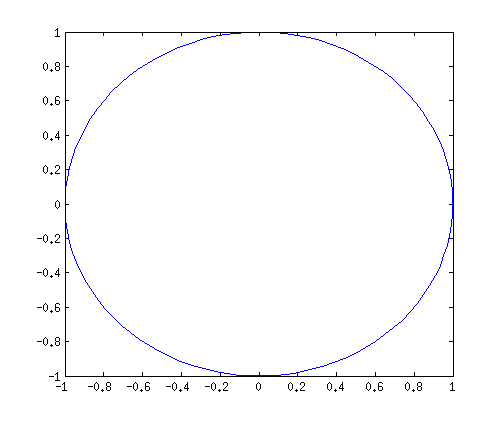
\includegraphics[scale=0.7]{26_1}$\\
\end{center}

$$\vec{S}(z=2m)=H_{0}^{2}|Z|e^{4\alpha}\vec{i_{z}}(\sin(\omega t - 2\beta + \cfrac{\pi}{6})\sin(\omega t - 2\beta) + \cos(\omega t - 2\beta)\cos(\omega t - 2\beta + \cfrac{\pi}{6}) )$$

\end{solution}
